% !TeX program = pdfLaTeX
\documentclass[12pt]{article}
\usepackage{amsmath}
\usepackage{amsthm}
\usepackage{graphicx,psfrag,epsf}
\usepackage{enumerate}
%\usepackage[numbers]{natbib}
\usepackage[nomarkers]{endfloat}
\usepackage{natbib}
\setcitestyle{numbers} 
\makeatletter % Reference list option change
\renewcommand\@biblabel[1]{#1. } % from [1] to 1
\makeatother %

\usepackage{booktabs}
\usepackage{longtable}
\usepackage{array}
\usepackage{adjustbox}
\usepackage{multirow}
\usepackage{subfig}
\usepackage[table,xcdraw]{xcolor}
\usepackage{wrapfig}
\usepackage{float}
%\usepackage{colortbl}
\usepackage[colorlinks]{hyperref}
\hypersetup{
  colorlinks=true,
  citecolor=black,
  linkcolor=black,
  urlcolor=blue}
  
\usepackage{pdflscape}
\usepackage{tabu}
\usepackage{threeparttable}
\usepackage{url} % not crucial - just used below for the URL

\usepackage{etoolbox}% http://ctan.org/pkg/etoolbox
\makeatletter
\patchcmd{\subsection}{\bfseries}{\relax}{}{}% Non-bold \subsection
\patchcmd{\subsubsection}{\bfseries}{\relax}{}{}% Non-bold \subsection
\makeatother


%\pdfminorversion=4
% NOTE: To produce blinded version, replace "0" with "1" below.
\newcommand{\blind}{0}

% DON'T change margins - should be 1 inch all around.
\addtolength{\oddsidemargin}{-.5in}%
\addtolength{\evensidemargin}{-.5in}%
\addtolength{\textwidth}{1in}%
\addtolength{\textheight}{1.3in}%
\addtolength{\topmargin}{-.8in}%

\newenvironment{definition}[1]% environment name 
{% begin code 
  \par\vspace{.75\baselineskip}\noindent 
  \textbf{Definition (#1)}\begin{itshape}% 
  \par\vspace{.5\baselineskip}\noindent\ignorespaces 
}% 
{% end code 
  \end{itshape}\ignorespacesafterend 
}

\providecommand{\tightlist}{%
  \setlength{\itemsep}{0pt}\setlength{\parskip}{0pt}}

\begin{document}

\def\spacingset#1{\renewcommand{\baselinestretch}%
{#1}\small\normalsize} \spacingset{1}



%%%%%%%%%%%%%%%%%%%%%%%%%%%%%%%%%%%%%%%%%%%%%%%%%%%%%%%%%%%%%%%%%%%%%%%%%%%%%%

\if0\blind
{
  \title{\bf A Robust Approach to Automatically Locating Grooves in 3D Bullet Land
Scans}

  \author{
        Kiegan Rice \thanks{We would like to thank the efforts of the Center for Statistics and
Applications in Forensic Evidence (CSAFE) and the Roy J. Carver High
Resolution Microscopy lab in scanning the Hamby set 44 and providing the
scans to us. This work was partially funded by the Center for Statistics
and Applications in Forensic Evidence (CSAFE) through Cooperative
Agreement No.~70NANB15H176 between NIST and Iowa State University, which
includes activities carried out at Carnegie Mellon University,
University of California Irvine, and University of Virginia.} \\
    Department of Statistics, Iowa State University\\
     and \\     Ulrike Genschel \\
    Department of Statistics and the Center for Statistics and Applications
    in Forensic Evidence (CSAFE), Iowa State University\\
     and \\     Heike Hofmann \\
    Department of Statistics and the Center for Statistics and Applications
    in Forensic Evidence (CSAFE), Iowa State University\\
      }
  \maketitle
} \fi

\if1\blind
{
  \bigskip
  \bigskip
  \bigskip
  \begin{center}
    {\LARGE\bf A Robust Approach to Automatically Locating Grooves in 3D Bullet Land
Scans}
  \end{center}
  \medskip
} \fi

\bigskip
\begin{abstract}
Land engraved areas (LEAs) provide evidence to address the same
source-different source problem in forensic firearms examination.
Advances in technology have led to new research on applying
image-analysis algorithms to the automated, quantitative analysis of
bullet evidence. One prominent example is an algorithm developed by Hare
et. al \citep{Hare1} based on 3D imaging data of LEAs. Currently
accepted best practice for collecting 3D images of bullet LEAs requires
capturing portions of the neighboring groove engraved areas (GEAs).
Analyzing LEA and GEA data separately is imperative to achieve high
accuracy and precision in subsequent feature comparisons. However,
existing standard statistical modeling techniques fall short when
applied to the atypical structure of 3D bullet data, often failing to
adequately separate LEA and GEA data. We developed a method for
automated removal of GEA data based on robust locally weighted
regression. This automated method was tested on high resolution 3D scans
of LEAs from Hamby set 44. This separation method outperforms current
methods at separating LEA and GEA data.
\end{abstract}

\noindent%
{\it Keywords:} land engraved areas (LEAs), groove engraved areas (GEAs), 3D scans, bullet identification, automatic matching
\vfill

\newpage
\spacingset{1.45} % DON'T change the spacing!

\newcommand{\hh}[1]{{\color{orange}{#1}}}
\newcommand{\kr}[1]{{\color{teal}{#1}}}
\newcommand{\ug}[1]{{\color{purple}{#1}}}

\section{Reviewer Comments}

Below are the reviewer comments with proposed responses. Proposed
changes in accordance with reviewer comments within the text are colored
teal.

\subsection{Reviewer 1}

\begin{enumerate}
\def\labelenumi{\arabic{enumi}.}
\tightlist
\item
  ``Currently accepted best practice\ldots{}''

  \begin{itemize}
  \tightlist
  \item
    We have rephrased in accordance with the reviewer's comment.
  \end{itemize}
\item
  ``2D crosscuts'' should be ``1D profiles''.

  \begin{itemize}
  \tightlist
  \item
    Profiles are recorded in two dimensions - location and height.
    Traditionally in imaging, 3D topographies such as these might be
    considered 2.5-D, which would make profiles 1.5-D. In order to avoid
    discussion of dimensionality here, we choose to remove dimension
    entirely and refer to them as simply ``crosscuts'' and
    ``profiles''.\\
  \end{itemize}
\item
  Duplicate paragraph.

  \begin{itemize}
  \tightlist
  \item
    Noted and removed.
  \end{itemize}
\item
  Describe rollapply, whether it is publicly available, etc.

  \begin{itemize}
  \tightlist
  \item
    An additional paragraph describing the rollapply method and where it
    is available has been added to the background section.
  \end{itemize}
\item
  Figure 8 (boxplots).

  \begin{itemize}
  \tightlist
  \item
    We have rewritten to clarify what we are plotting. The description
    of Figure 8 within the text has been updated to clarify this point,
    as well as the figure caption.
  \end{itemize}
\item
  Figure 9/Table 1 are duplicated.

  \begin{itemize}
  \tightlist
  \item
    They are in fact based on the same numbers. However, the figure
    gives an overview of trend while the table provides the specific
    quantitative information. For this reason, we believe they both
    provide the audience with useful insight. A sentence clarifying that
    they are sourced from the same information has been added.
  \end{itemize}
\item
  Defend choice of cutoffs for results.

  \begin{itemize}
  \tightlist
  \item
    The binning could be done differently. What we want to see is
    essentially a rough categorization of different levels of deviation
    from the ``ground truth'' shoulder location. To clarify this, we
    have renamed the categories as ``small deviation'', ``medium
    deviation'', and ``large deviation''.
  \end{itemize}
\item
  X3P should be all caps

  \begin{itemize}
  \tightlist
  \item
    The ISO standard, referenced in the ``Data Source'' section, defines
    x3p as ``x3p'', with lowercase ``x'' and ``p''.
  \end{itemize}
\item
  Caliber, ammo brand, bullet material

  \begin{itemize}
  \tightlist
  \item
    We have updated the data source section to include this information.
  \end{itemize}
\item
  Why was 0.645 chosen as the resolution?

  \begin{itemize}
  \tightlist
  \item
    This is the resolution of our instrument at 20x magnification, so we
    are bound by 0.645. For reference, Hamby sets scanned at NIST and
    posted publicly on the NIST Ballistics and Toolmark Research
    Database (NBTRD) are gathered at a resolution of 1.5625
    microns/pixel. Our machine's resolution is higher than that.
  \end{itemize}
\item
  Is rollapply only other method? Is it current-best?

  \begin{itemize}
  \tightlist
  \item
    Rollapply is the only other automated approach available in the
    literature for methods which perform LEA-to-LEA comparisons.
  \end{itemize}
\item
  Fig. 5 and 6 should be same data, or clarify if they are not.

  \begin{itemize}
  \tightlist
  \item
    We have added information about which LEA is shown in Figures 5, 6,
    and 7 for clarity.
  \item
    Figure 5 has also been updated to be the same LEA data as Figures 5
    and 6 for clarity.\\
  \end{itemize}
\item
  Why is right shoulder harder to find?

  \begin{itemize}
  \tightlist
  \item
    We added additional details to support our hypothesis on this point.
  \end{itemize}
\end{enumerate}

\subsection{Reviewer 2}

\begin{enumerate}
\def\labelenumi{\arabic{enumi}.}
\item
  Title is confusing

  \begin{itemize}
  \tightlist
  \item
    We have updated the title for clarification.
  \end{itemize}
\item
  ``Visual feature comparison'' vs ``pattern matching''

  \begin{itemize}
  \tightlist
  \item
    We use ``visual feature comparison'' over ``pattern matching''
    because we want to emphasize the process of comparison, not the
    result. However, for clarification, we have re-worded to simply
    ``visual comparison''.
  \end{itemize}
\item
  ``Striated tool marks''

  \begin{itemize}
  \tightlist
  \item
    Reworded to use the phrase striated tool marks instead of
    striations.
  \end{itemize}
\item
  Citation for ``same source-different source problem''.

  \begin{itemize}
  \tightlist
  \item
    Added a citation.
  \end{itemize}
\item
  Spell out LEA. Use ``toolmarks produced on fired bullets''.

  \begin{itemize}
  \tightlist
  \item
    Spelled out LEA on its first appearance.
  \item
    Added a statement to clarify that we are referring to toolmarks on
    fired bullets.
  \end{itemize}
\item
  ``3rd paragraph\ldots{}''

  \begin{itemize}
  \tightlist
  \item
    We are assuming you would like us to rephrase. We have done so.
  \end{itemize}
\item
  ``Impressed'' should be ``engraved''.

  \begin{itemize}
  \tightlist
  \item
    You are correct. We have rephrased.
  \end{itemize}
\item
  ``Automated Computer Vision Techniques''

  \begin{itemize}
  \tightlist
  \item
    We were referring to automated computer vision techniques in
    general. However, to clarify for this specific application, we have
    rephrased.
  \end{itemize}
\item
  ``Data source\ldots{}''

  \begin{itemize}
  \tightlist
  \item
    Yes, there are some papers that assume operators will manually trim.
    This is not what the Hare et. al.~paper does. Rollapply is an
    automated approach to this in that paper.
  \end{itemize}
\item
  ``Tank rash''

  \begin{itemize}
  \tightlist
  \item
    Have rephrased.\\
  \end{itemize}
\item
\item
  Misread of process in Fig. 7

  \begin{itemize}
  \tightlist
  \item
    Note that our process, described step-by-step on page 8, is simply
    to identify shoulder locations. All LEA data inside those shoulder
    locations are preserved and remain as part of the data included in
    further analysis.
  \item
    Lines to reference where identified shoulder locations would be have
    been added to Figs. 6d and 7d, and clarifications have been added to
    the figure captions.
  \end{itemize}
\item
  Bullets with smooth GEA

  \begin{itemize}
  \tightlist
  \item
    This particular method is meant for sharp-edged rifling. Smooth GEAs
    would not cause the same structural issues as sharp-edged rifling.
    In downstream analysis, a LOESS fit to the bullet structure can
    capture the more gradual changes present with a smooth GEA and still
    produce a useful signature.
  \end{itemize}
\item
  Shoulders not aligned along longitude could cause a problem

  \begin{itemize}
  \tightlist
  \item
    We have noted this limitation in our conclusions section.
  \end{itemize}
\item
  ``MUST rely on operator to manually crop''

  \begin{itemize}
  \tightlist
  \item
    There is not really a comment or suggested change that we can
    address.
  \end{itemize}
\item
  ``Comparison of manually cropped vs.~automated using CCF''
\item
  ``Diversity in scan sets''

  \begin{itemize}
  \item
    {\color{teal}{We have added an additional test set, Houston-test, to our results section. This has also been detailed in the data source section.}}
  \item
    {\color{teal}{The figures have been updated to include the Houston-test set, but the table has not. Should the table for Hamby and Houston be kept separate?}}
  \end{itemize}
\end{enumerate}

\section{Background}

Forensic firearms examiners analyze bullets through a process of
{\color{teal}{visual comparison}} to determine whether two bullets
originate from the same source. Two bullets in question are placed under
a comparison microscope and firearms examiners evaluate similarities and
differences between
{\color{teal}{striated toolmarks produced on fired bullets from rifled barrels. The assessment of these patterns follows}}
the AFTE Theory of Identification \citep{AFTE} guidelines resulting in a
decision about whether both bullets were fired through the same gun
barrel. In forensic science, this problem is known as the \emph{same
source-different source problem} {\color{teal}{[see @Ommen1]}} and it
focuses on establishing quantitative evidence whether two bullets were
fired through the same gun barrel.

Recent advances in technology, particularly wider access to high
resolution 3D microscopy tools, have led to an increase in research on
image-analysis algorithms for automated, quantitative analyses of bullet
evidence. The introduction of such scanning technology to the field of
forensic science allows for capture of high resolution 3D images of
bullet land engraved areas (LEAs), depicted in \autoref{microscope}
\citep[see][]{DeKinder1, DeKinder2, Bachrach1}. The resulting 3D images
have since been used in the development of several novel methods for
automated comparison of land engraved areas
\citep[e.g.][]{Ma1, Chu1, Chu2, Hare1}.

\begin{figure}

{\centering 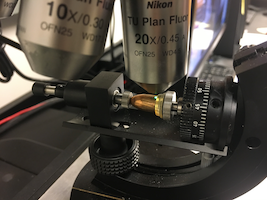
\includegraphics[width=0.48\textwidth]{./images/microscope-small} 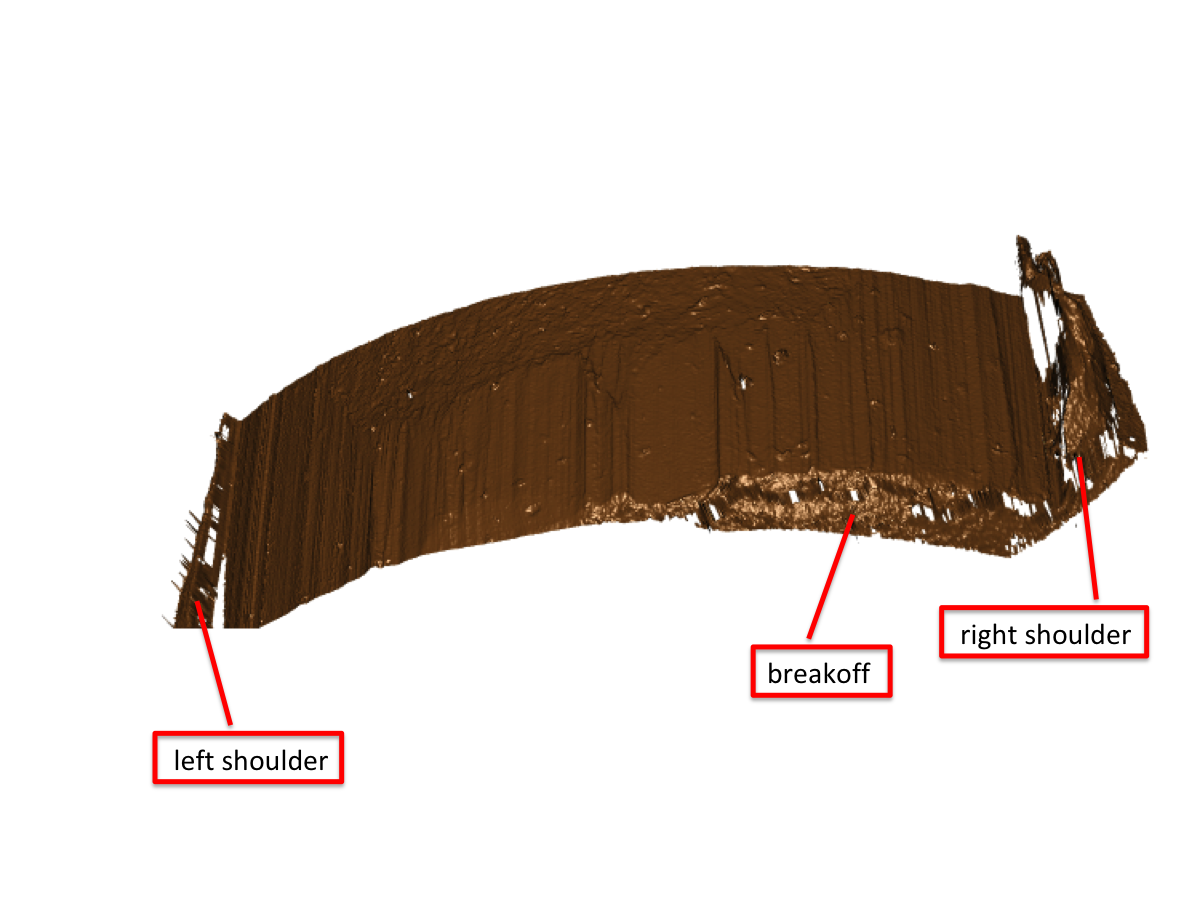
\includegraphics[width=0.48\textwidth]{./images/HS44-Br1-B1-L2-annotated} 

}

\caption{\label{microscope}(Left) Close-up view of a bullet staged in a confocal light microscope. The green light marks the focal view of the capture area. (Right) Computer-rendered image of the scanned land engraved area with prominent striation marks. Breakoff is seen visually on the bottom right hand side of the scan.}\label{fig:microscope}
\end{figure}

In this paper, we will focus only on barrels with traditional
sharp-edged lands and grooves (i.e., no polygonal rifling). Sections of
the bullet that make
{\color{teal}{contact with high points inside the barrel are called land engraved areas (LEAs) and alternate with low points called groove engraved areas (GEAs).}}
Micro imperfections in the barrel introduce striae on the bullet during
the firing process. The resulting striation marks provide evidence to
address the same source-different source problem. A guiding principle in
forensic firearms analysis is that two bullets fired through the same
barrel will bear more similar striation marks on their LEAs than two
bullets fired from different barrels. \citet{Hare1} proposes a matching
algorithm based on 3D imaging data of LEAs. Horizontal slices of the 3D
images, called crosscuts, provide a detailed representation of striae
engraved on the surface at a horizontal cross-section of each LEA. A
current limitation of this algorithm is that it cannot deal with a mix
of striae from both LEA and GEAs. For the human visual system,
separating the two areas is straightforward. However, the same cannot be
said for automated {\color{teal}{computer toolmark comparison}}
techniques.

A correct identification of LEAs is vital to achieve high accuracy and
precision in the subsequent downstream analysis and our goal is to
present and discuss different automated methods for identifying
so-called \emph{shoulder locations}, the locations at which the land
engraved areas end and the groove engraved areas begin.

{\color{teal}{The best currently available method to identify these shoulder locations is the ``rollapply" method proposed by @Hare1. This method is publicly available through the \texttt{bulletxtrctr} package for the open source statistical computing language \texttt{R}. The authors propose first applying a rolling average to each profile to smooth out bumps in data, followed by identifying the local minima closest to the edges of each smoothed profile.}}

The structure of the paper is as follows: a description of the data
storage format and data set, an explanation of methodology to predict
shoulder locations, and finally an illustration of improved prediction
accuracy results.

\section{Data Source}

All currently published automated methods rely on high resolution 3D
scans of bullet land engraved areas.
{\color{teal}{Our approach to the collection of}} 3D images of bullet
LEAs requires that bullets are staged such that striae appear vertically
in the scan. Scanning across the LEA must begin and end in the
neighboring groove engraved areas as shown in \autoref{fig:LEA}. Parts
of the breakoff are captured as a visual reference for orientation (see
\autoref{fig:microscope}).

\begin{figure}
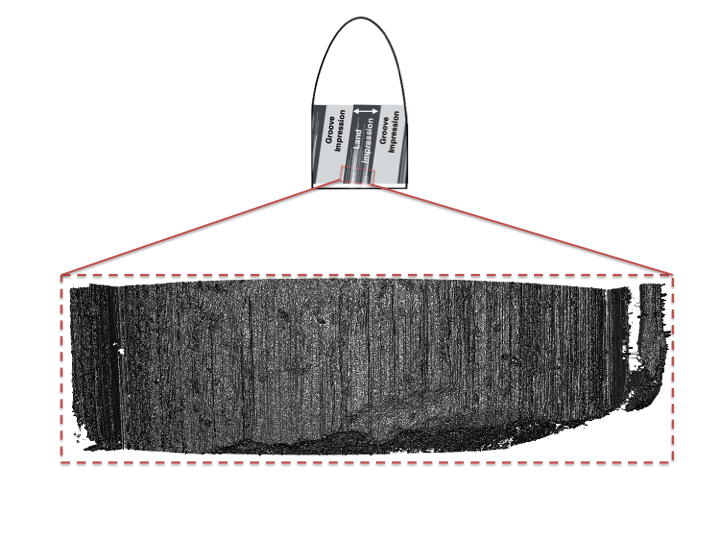
\includegraphics[width=\textwidth]{./images/3d_plot_top_context_breakoff} \caption{\label{LEA}Visualization of 3D data collected through high resolution scanning of a land engraved area. Striations on the surface of the object can be seen by viewing this data from "above", as presented here.}\label{fig:LEA}
\end{figure}

Scans are exported from the microscope as x3p files, conforming to the
ISO5436-2 standard \citep{ISO5436}. Each scan is recorded as a matrix of
prespecified \((x,y)\) locations with a measured relative height value
\(z\) for each \((x,y)\) location on the LEA.

The algorithm proposed by \citet{Hare1} uses so-called crosscuts, height
measurements along \(x\) for a fixed \(y\). Removal of the overall curve
of the bullet -- the global structure captured in the 3D scanning
process -- transforms these crosscuts into to what \citet{Hare1} refer
to as \emph{signatures} (see \autoref{fig:process}). The assessment of
similarity between two LEAs is then based on a set of extracted features
such as cross-correlation function, number of consecutively matching
striae \citep[see][]{Biasotti} and maximum number of consecutively
non-matching striae. Successful extraction of this set of features
depends on how well we can remove the global bullet structure to
translate from a crosscut to the corresponding signature.

\begin{figure}
\begin{minipage}[b]{0.45\linewidth}
    \raggedleft
    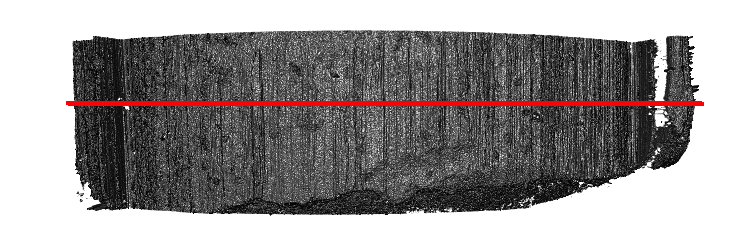
\includegraphics[width=\textwidth]{images/3d_plot_top_crosscut}
    \centering
    Step 1: 3D scan with identified horizontal crosscut
\end{minipage}
\hspace{.5cm}
\begin{minipage}[b]{0.45\linewidth}
    \raggedright
    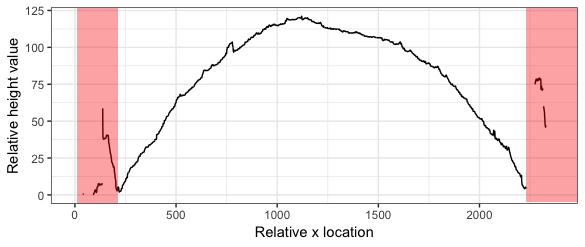
\includegraphics[width=\textwidth]{images/profile_paper}
    \centering
    Step 2: Horizontal crosscut with identified GEA data
\end{minipage}\\

\vspace{.3cm}
\begin{minipage}[b]{0.45\linewidth}
    \raggedleft
    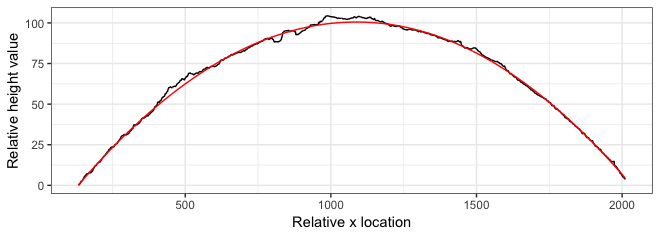
\includegraphics[width=\textwidth]{images/profile_paper_loess}
    \centering
    Step 3: Non-parametric curvature estimation
\end{minipage}
\hspace{.5cm}
\begin{minipage}[b]{0.45\linewidth}
    \raggedright
    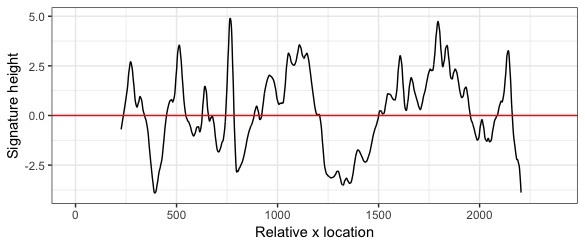
\includegraphics[width=\textwidth]{images/signature_paper}
    \centering
    Step 4: Extracted LEA signature
\end{minipage}
\caption{The process of extracting a signature from a 3D LEA scan described by \cite{Hare1}. GEA removal between Steps 2 and 3 is critical to ensure precise signature extraction.}  
\label{fig:process}
\end{figure}

In the following, we are introducing and comparing two methods for
identifying shoulder locations. In order to assess the performance of
these methods, we are applying both methods on 3D scans of LEAs from
Hamby set 44 \citep{Hamby} {\color{teal}{and the Houston-test set}}.
Each Hamby set consists of 35 {\color{teal}{Winchester 9mm copper}}
bullets fired from 10 consecutively rifled Ruger P-85
{\color{teal}{9mm Luger}} barrels.
{\color{teal}{The Houston-test set consists of XXX bullets fired from XXX type of barrels...}}

Each fired bullet in Hamby Set 44 and Houston-test set has 6 LEAs; every
LEA was scanned for each of the 35 {\color{teal}{plus houston-test}}
bullets, producing data for 210 individual LEAs. Two LEAs from Hamby Set
44 -- Barrel 9, Bullet 2, Land 3 and Questioned Bullet L, Land 5 -- were
removed from consideration
{\color{teal}{because they were deemed unsuitable for comparison. These two LEAs contained significant abrasians created by contact with the bottom of a water recovery tank after exiting the barrel. These abrasians are thus marks present on the LEAs that are not due to contact with the barrel itself}}.

All 3D scans of Hamby Set 44 and Houston-test were captured at Iowa
State University's Roy J.~Carver High Resolution Microscopy Facility
with a Sensofar Confocal light microscope at 20 times magnification
resulting in a resolution of 0.645 microns per pixel (1 micron =
1\(\mu\)m = 0.001mm). Physically, each land is approximately 2
millimeters in width; as such, data structures for a single LEA can
contain more than 3 million individual data points.

\begin{figure}
\centering
\includegraphics{writeup_files/figure-latex/prof-1.pdf}
\caption{\label{prof}The black points show measured heights for a single
crosscut of a 3D LEA scan. The main data structure, located in the
center, is comprised of the land engraved area. The groove engraved
areas are found on the left and right sides of the crosscut. The lines
show fits of two non-parametric LOESS smooths, with and without GEA
data. When GEA data is included, the smooth fails to estimate the main
LEA structure near the boundaries. The LEA pictured here is Hamby 44,
Barrel 10, Bullet 2, Land 2.}
\end{figure}

Data used to assess performance of the two methods consist of crosscuts
gathered from the 3D scans, as shown in \autoref{prof}.

\section{Methodology}

The structure in the crosscuts is dominated by the curvature of the
physical object (the bullet). To assess the similarity of features from
two land engraved areas, this curvature has to be removed.

Non-parametric methods suggested in the literature, such as a LOESS fit
\citep{Hare1} or a Gaussian filter \citep{Chu1} are effective for
removing the curvature to extract a signature. However, they are prone
to boundary effects, which cause mischaracterizations of data patterns
near the boundaries of the data domain. In the case of crosscuts, the
boundaries are often dominated by values originating from the GEA
structure. This structure exaggerates existing boundary effects because
GEAs introduce a secondary structure different from the main curvature
of the LEA, as shown in \autoref{prof} and \autoref{groove-no-groove}.
\autoref{prof} shows how much a non-parametric LOESS fit is affected by
including GEA data. \autoref{groove-no-groove} illustrates the effect
the inclusion of the same has on extracted signatures. If included, GEA
data result in strong boundary effects in the signatures. Statistically,
GEA data introduce outliers into the LEA data. In the next sections, we
introduce two methods for fitting the LEA structure. Both methods aim to
describe the relationship between horizontal position and relative
height on a crosscut. While the two approaches differ in methodology,
they are both rooted in the ability to mitigate potential influence
caused by outlying data.

\begin{figure}
\centering
\includegraphics{writeup_files/figure-latex/groove-no-groove-1.pdf}
\caption{\label{groove-no-groove}An example of the impact failure to
remove GEA data can have on an extracted signature. Even though there
are only very few points in the GEA structure, the extracted signatures
are dominated by boundary effects. The LEA pictured here is Hamby 44,
Barrel 10, Bullet 2, Land 2.}
\end{figure}

In the following, we will describe the horizontal position on a crosscut
of a scan as \(x_i\) and measured relative height as \(z_i\), where
\(i = 1, \dots, n\), the number of data points along a crosscut.

\subsection{Robust Linear Models}

A natural candidate for a curved structure is a quadratic linear model
of the form

\[
z_i = \beta_0 + \beta_1x_i + \beta_2 x_i^2 + \epsilon_i,
\] where all error terms \(\epsilon_i\) are considered independent and
normally distributed with mean \(0\) and variance \(\sigma^2\).
Parameter values of \(\beta_0, \beta_1, \beta_2\) are estimated by
finding the values which minimize:

\[\arg\min_{\mathbf{\beta}} \sum_{i=1}^n \left(z_i - (\beta_0 + \beta_1x_i + \beta_2x_i^2)\right)^2,\]
the vertical squared distance between each measured height value and the
fitted curve. \autoref{lms} shows that the presence of outliers near the
boundaries pulls the resulting curve upwards towards groove engraved
area data.

Alternatively, the curve can be fit by minimizing the absolute
deviations in place of squared deviations:

\[\arg\min_{\mathbf{\beta}} \sum_{i=1}^n \left|z_i - (\beta_0 + \beta_1x_i + \beta_2x_i^2) \right|.\]

This method of minimization is less influenced by large outliers present
in the GEA data and the resulting model is known as a robust linear
model.

Estimation based on taking squared deviations seeks to balance the fit
between the LEA structure and the GEA structure, resulting in a fit
which compromises between both structures without adequately fitting
either. The use of absolute deviations reduces the degree of compromise
in favor of fitting the majority structure, here LEA. \autoref{lms}(a)
and (c) show the fitted curves from each model framework.
\autoref{lms}(b) and (d) display the differences between predicted
height and observed height at each location \(x_i\), known as the
observed model residuals \(e_i\). We will utilize the observed residuals
to separate the two structures. The robust model in \autoref{lms} fits
the LEA structure more closely and better captures the curvature,
allowing for a more accurate separation between GEA and LEA structures.

\begin{figure}
\centering
\includegraphics{writeup_files/figure-latex/lms-1.pdf}
\caption{\label{lms}Example of a quadratic linear model fit and
resulting residuals (a, b) compared to a robust quadratic linear model
fit and residuals (c, d) for a single profile. The robust model is able
to more effectively capture the curved structure of the LEA without
being influenced by the GEA. The dashed horizontal line in (d) is drawn
at 4 x MAD. Values above the dashed line are considered outliers. The
vertical lines in (d) are drawn where the left and right shoulder
locations would be identified. The LEA pictured here is Hamby 44, Barrel
10, Bullet 2, Land 2.}
\end{figure}

Because the robust approach results in residual values scattered near
zero in the land engraved area and larger, mostly positive residuals in
the groove engraved area, we will use high residual magnitude as an
indicator of GEA membership (see \autoref{lms}). High residual magnitude
is determined using the median absolute deviation (MAD) of all residuals
from a crosscut.

The MAD is a robust metric for the spread of data, similar to the
standard deviation. It is preferable to the standard deviation to
quantify the spread in situations with large outlying observations, such
as the residuals in the groove engraved area.

Let \(m\) denote the median function. Then the MAD is defined as
\[ MAD(\mathbf{e}) = m(|e_i- m(\mathbf{e})|) \quad \forall\ e_i \in \mathbf{e}.\]
Any residual value larger than \(4 \times\)MAD is considered an outlier
and likely a member of the GEA structure.

Shoulder location predictions are then calculated for each crosscut in
the following manner (\textbf{Linear Shoulder Location Prediction}):\\

\begin{enumerate}
\item Fit a robust linear model of order 2 (i.e., quadratic) to the crosscut.   
\item Calculate a residual value $e_i$ for each data point on the crosscut.  
\item Calculate the residual median absolute deviation (MAD) for the crosscut.  
\item Remove all data points on the crosscut with a residual magnitude greater than $4 \times$MAD.  
\item Identify the minimum $x_{L}$ and maximum $x_{R}$ of the remaining $x_i$ values. Then, $x_L$ and $x_R$ are the predicted left and right shoulder locations for that crosscut.   
\end{enumerate}

\subsection{Robust LOESS}

One of the drawbacks of the linear approach is its rigidity in the shape
of the curve. Locally weighted regression, known as LOESS, is a more
flexible approach. This is advantageous when working with bullets, as it
is unrealistic to expect a circular shape to remain after the bullet has
been subjected to the forces of a gun barrel.

LOESS models estimate a predicted value \(\widehat{z}_i\) for each
height \(z_i\) corresponding to location \(x_i\) by estimating values
\(\beta_0, \beta_1\) which minimize

\begin{equation}\label{eq:RobLOESS} \arg\min_{\mathbf{\beta}} \sum_{k=1}^n w_k(x_{i})\left(z_{k} - (\beta_0 + \beta_1x_k)\right)^2,\end{equation}

where \(w_k(x_i)\) is a weight assigned to each data point \(x_k\) based
on its proximity to \(x_i\). Weights \(w_k\) decrease as the distance to
\(x_i\) increases, so that data points closest to \(x_i\) influence the
prediction \(\widehat{z}_i\) most. A LOESS model can also be described
as a non-parametric weighted average of many parametric models fit to
subsets of the data.

Although this approach allows for greater flexibility, LOESS models are
affected more by GEA structures than robust linear models are. Data
points near and in the GEA structure are most influenced by other GEA
data rather than the overall global structure. This results in a set of
predictions which misrepresents much of the data near the boundaries
(see \autoref{loess}).

Similar to the linear approach, there exists a robust approach to LOESS
to adjust for these boundary effects.

The robust approach to LOESS uses an iterative re-weighting process to
reduce the influence of outlying data points \citep[see][]{Cleveland1}.
First, an initial LOESS is fit. This step is followed by a
redistribution of the weights \(w_k(x_i)\) based on residual values,
\(e_i = (z_i - \widehat{z}_i)\). New weights are calculated as
\[\left(1-\left(\frac{e_k}{6\times MAD}\right)^2\right)^2 \times w_k(x_i) \quad \quad \mbox{if}\quad \ \left|\frac{e_k}{6\times MAD}\right| < 1,\]
else, weights are set to 0. These new weights are re-applied in
(\ref{eq:RobLOESS}) and updated predictions are obtained. This reduces
the influence of data points with large residual values \(e_k\) in
subsequent iterations. In the context of LEA crosscuts, this
re-weighting reduces the influence of GEA data.

A robust LOESS model which accurately fits the LEA structure should
result in a similar residual structure as that expected for the robust
linear model: small residuals scattered near zero for \(x_i\) locations
in the land engraved area, and positive, possibly large residuals for
\(x_i\) locations in the groove engraved areas. The increased
flexibility of LOESS models lead to a closer fit to the curvature and
thus the robust LOESS more reliably results in the aforementioned
residual pattern. We can thus use a lower cutoff for separation of the
residuals via magnitude. A cutoff that performs well on the Hamby set 44
is twice the median absolute deviation (\(2 \times MAD\)).

\begin{figure}
\centering
\includegraphics{writeup_files/figure-latex/loess-1.pdf}
\caption{\label{loess}Example of a LOESS model fit and residuals (a, b)
compared to a robust LOESS model fit and residuals (c, d) for a single
profile. The robust model is again able to more effectively capture the
curved structure of the LEA without being influenced by the GEA. The
dashed line in (d) represents a cutoff of 2 x MAD. Values above the
dashed line are considered outliers. The vertical lines in (d) are drawn
where the left and right shoulder locations would be identified. The LEA
pictured here is Hamby 44, Barrel 10, Bullet 2, Land 2.}
\end{figure}

Shoulder location predictions are calculated for each crosscut in the
following manner (\textbf{LOESS shoulder location prediction}):

\begin{enumerate}
\item Fit a robust LOESS model to the crosscut \citep{locfit}.
\item Calculate a residual value $e_i$ for each data point on the crosscut.  
\item Calculate the residual median absolute deviation (MAD) for the crosscut.  
\item Remove all data points on the crosscut with a residual magnitude greater than $2 \times$MAD.  
\item Identify the minimum $x_{L'}$ and maximum $x_{R'}$ of the remaining $x_i$ values. Then, $x_{L'}$ and $x_{R'}$ are the predicted left and right shoulder locations for that crosscut.   
\end{enumerate}

\section{Results}

To quantitatively assess the predictive ability of the two alternative
models, we first identified ``ground truth'' of shoulder locations by
visual inspection for each of the 208 crosscuts in Hamby set 44
{\color{teal}{and each of the 414 crosscuts in Houston-test}}.

As a performance measure, we define the error as the ``area of
misidentification'', i.e., the area of each crosscut which is identified
incorrectly by the method. This metric is calculated for the left
shoulder location as:

\[ \widehat{A}_{jL} = \sum_{e_{ij} \in \widetilde{X}_{jL}} \left|e_{ij} \right| \times \left(x_{i+1} - x_i \right),\]
where \(\widetilde{X}_{jL}\) is the set of points in crosscut \(j\) that
fall between the predicted and actual left shoulder location, \(e_{ij}\)
corresponds to the residual value at location \(x_i\) from the robust
LOESS fit to crosscut \(j\), and \((x_{i+1} - x_i)\) is the distance
between two subsequent locations in the crosscut. For the scans of Hamby
set 44 {\color{teal}{and Houston-test}}, this distance is equal to
\(0.645 \mu m\) for all locations.

Similarly, the area is calculated for the right shoulder location as:

\[ \widehat{A}_{jR} = \sum_{e_{ij} \in \widetilde{X}_{jR}} \left|e_{ij} \right| \times \left(x_{i+1} - x_i \right),\]
where \(\widetilde{X}_{jR}\) is the set of points in crosscut \(j\) that
fall between the predicted and actual right shoulder location.

Both the left and right areas of misindentification are thus in terms of
microns and represent the area of loss we incur from incorrectly
identifying a shoulder location.

Quantifying the results as an area is preferable to a distance metric as
it captures not only the width of the profile area that is
misidentified, but also the relative heights of the data. Larger
misidentified areas indicate larger portions of the GEA remain included
in a profile, and thus signal an area which is more likely to have
influence on an extracted signature. Smaller areas of misidentification
suggest minimal loss is incurred, and these areas will have minimal
effect on an extracted signature.

An area of misidentification was calculated separately for the left hand
side and right hand side predictions for each of the 208
{\color{teal}{+414}} profiles in the data set, where predictions were
based on the Robust Linear Model and Robust LOESS methods, as well as
the Rollapply method suggested in \citet{Hare1}.

To assess the performance of all three methods, we consider the
distribution of the areas of misidentification across all 208
{\color{teal}{+414}} lands of Hamby set 44
{\color{teal}{and Houston-test}}.
{\color{teal}{\autoref{results1} presents each distribution as a boxplot. The box encompasses the middle 50\% of values, spanning the 25th to 75th percentile. The line inside each box represents the median value, and individual data points are unusually large values we call outliers.}}
A distribution starting at or close to zero with minimal spread is ideal
as this suggests many of the predicted shoulder locations are very close
to the manually identified locations, and predictions are removing many
of the outlying GEA points. A distribution with a wider spread or many
high, outlying areas of misidentification suggests a greater degree of
uncertainty and inaccuracy for a particular method.
{\color{teal}{Some of the outliers are so extreme, statistics appear very close to one another or on top of each other.}}

\begin{figure}
\centering
\includegraphics{writeup_files/figure-latex/results1-1.pdf}
\caption{\label{results1}Distribution, presented here as a boxplot, of
areas of misidentification for rollapply (data smoothing) method, robust
linear model method, and robust LOESS method, separated by left and
right shoulder locations. A dense distribution with few high values
indicates good performance across the LEAs in the data set.}
\end{figure}

Because the raw distributions are difficult to visually compare due to
extreme outliers, we categorized areas of misidentification as
{\color{teal}{small, medium, and large deviations. Scores under 100 are considered small deviations, scores between 100 and 1000 are medium, and scores above 1000 are considered large deviations (see \autoref{results2}). Cases with large deviations are the most likely to cause poor or flawed results in subsequent analyses.}}
Note that \autoref{results2} and \autoref{results-table} are based on
the same numbers but provide two different presentations of the results.

It is important to note that different results are expected for the left
and right shoulder locations. Within Hamby set 44, almost all scans have
a well-defined left groove. Left here is defined as visually left on the
scan; this is the side the scan begins on, so a well-defined distinction
between GEA and LEA is expected. Often, a less clear distinction is seen
on the right side of the scan, with sometimes no apparent shoulder
location visible.
{\color{teal}{This may be due to the left shoulder corresponding to the leading edge in the twist of a bullet as it is propelled through a gun barrel.}}
For this reason it is preferable to separate the left and right for
visual inspection of results; a method may excel on one side but fall
short on another.

\begin{figure}
\centering
\includegraphics{writeup_files/figure-latex/results2-1.pdf}
\caption{\label{results2}Distribution of areas of misidentification for
rollapply (data smoothing) method, robust linear model method, and
robust LOESS method, separated by left and right shoulder locations.
Areas of misidentification are placed into three categories: less than
100 microns (small deviations), between 100 and 1000 microns, and
greater than 1000 microns. A larger proportion of areas of
misidentification under 100 microns indicates good performance across
LEAs in the data set.}
\end{figure}

\begin{table}[]
\centering
\begin{tabular}{lrrr|rrr}
& \multicolumn{3}{c}{\textbf{Left Shoulder Location}} & \multicolumn{3}{c}{\textbf{Right Shoulder Location}} \\
\textbf{Method} & $(0,100)$ & $ (100, 1000) $ & $(1000, \infty)$ & $(0,100)$ & $ (100, 1000) $ & $(1000, \infty)$ \\ \hline
Rollapply & 86.54 & 8.17 & 5.29 & 52.88& 34.13&12.98  \\ \hline
Robust Linear Model & 78.85 & 13.94 & 7.21 & 62.50 & 30.77&6.73 \\ \hline
Robust LOESS & 94.23 & 5.29 & 0.48 & 73.08& 24.04&2.88\\ \hline
\end{tabular}
\caption{Table of results for areas of misidentification (in $\mu m^2$) resulting from automated shoulder location identification methods applied to Hamby set 44. Results are presented as percentage of shoulder location predictions which fall into each category: small deviations (less than 100), medium deviations (between 100 and 1000), and large deviations (greater than 1000).}
\label{results-table}
\end{table}

\section{Conclusions}

Both the robust linear model and robust LOESS approaches outperform
currently implemented solutions based on data smoothers for the right
shoulder location. Of the two, the robust LOESS approach clearly
outperforms the robust linear model. This hierarchy of performance is
well within expectation given the strength of robust approaches in
general as well as the flexibility of LOESS applied to this data type.
Robust LOESS also readily handles variation introduced in the process of
translating the physical bullet into a 3D object. If there is too much
variability in how the bullet is placed relative to the plane of
reference on the microscope, profiles can have tilted shapes relative to
the x-axis which a quadratic linear model would fail to address. In
these situations, LOESS excels.

While the proposed cutoff values as multiples of MAD work well on Hamby
set 44 {\color{teal}{and Houston-test}}, additional validation will need
to be executed on a wider variety of barrel types. Depth of striae,
physical size of bullet due to caliber, and non-traditional rifling
techniques may require alterations to this cutoff value.
{\color{teal}{LEAs with shoulders which are not aligned horizontally due to tild may also require slight alterations to the method.}}
In addition, a study of the effect of implementing robust LOESS shoulder
location identification on the downstream similarity assessment will
need to be completed. Due to increased accuracy of predicted shoulder
locations, the authors expect an increase in accuracy in bullet matching
algorithms. However, this will need to be validated on a variety of data
sets prior to implementation without human intervention in the automated
process.

\bibliographystyle{jfs-authoryear}
\bibliography{bibliography.bib}

\end{document}